\documentclass[11pt,aspectratio=169]{beamer}
\usepackage[T1]{fontenc}
\usepackage[utf8]{inputenc}
\usepackage{babel}
\babelprovide[main,import]{spanish}
\usepackage{lmodern,amsmath,amssymb,booktabs,array,tikz}
\definecolor{navy}{HTML}{17324D}
\definecolor{teal}{HTML}{168F8A}
\definecolor{pale}{HTML}{EDF5F7}
\setbeamercolor{normal text}{fg=navy,bg=white}
\setbeamercolor{structure}{fg=teal}
\setbeamercolor{frametitle}{fg=navy}
\setbeamercolor{title}{fg=navy}
\setbeamercolor{block title}{fg=navy,bg=pale}
\setbeamercolor{block body}{fg=navy,bg=pale}
\setbeamerfont{frametitle}{size=\Large,series=\bfseries}
\setbeamerfont{title}{size=\LARGE,series=\bfseries}
\setbeamerfont{block title}{series=\bfseries}
\setbeamertemplate{navigation symbols}{}
\setbeamertemplate{itemize item}{\color{teal}\small$\bullet$}
\setbeamertemplate{footline}{\hfill\color{navy}\scriptsize\insertframenumber\,/\,\inserttotalframenumber\hspace{6mm}\par\vspace{3mm}}
\setbeamersize{text margin left=9mm,text margin right=9mm}
\hypersetup{colorlinks=true,urlcolor=teal}
\newcommand{\notefoot}[1]{\vfill{\scriptsize\color{navy!75}#1}}
\newcommand{\lead}[1]{\begin{block}{}#1\end{block}}
\title{Fricciones de ejecución y desempeño\\de la inversión pública local}
\subtitle{Modelo económico de tesis - Vía B}
\author{Isis Milagros Roque Tinta}
\institute{Universidad del Pacífico - Modelamiento Económico}
\date{14 de octubre de 2026\\[6pt]\small\url{https://github.com/isisroquet-mi/ai-project}}
\begin{document}
\begin{frame}\titlepage\end{frame}

\begin{frame}{1. Pregunta de la tesis y pregunta teórica}
\textbf{Tesis:} ¿cómo se relaciona la pobreza distrital con la velocidad de ejecución y la variación de costos de proyectos de inversión pública local en el Perú?
\par\vspace{5mm}
\textbf{Vía B:} formular un mecanismo económico que sustente esa pregunta.
\lead{¿Cómo cambia la intensidad elegida cuando ejecutar es más difícil y cuándo aparece un sobrecosto respecto de lo previsto?}
\begin{itemize}
\item La tesis compara proyectos con controles territoriales, fiscales y de capacidad.
\item El modelo estudia una decisión y sus predicciones bajo supuestos explícitos.
\end{itemize}
\notefoot{Fuente: Bolo Añorga y Roque Tinta (2026), introducción y anexo 3.}
\end{frame}

\begin{frame}{2. El municipio elige cómo ejecutar el proyecto}
\begin{itemize}\setlength{\itemsep}{4mm}
\item \textbf{A1.} Proyecto viable que se ejecutará, de alcance y calidad fijos. El municipio minimiza su costo de implementación.
\item \textbf{A2.} Trabajo total normalizado a una unidad. Intensidad constante $e>0$ y duración $T(e)=1/e$.
\item \textbf{A3.} Costo base $M\geq0$, gasto de permanencia $F>0$ por periodo y fricción $\kappa>0$.
\end{itemize}
\lead{La decisión es la intensidad de ejecución. La aprobación del proyecto y el valor social de entregarlo antes quedan fuera de este problema.}
\notefoot{La ejecución dada es un supuesto analítico. La viabilidad, por sí sola, no implica ejecución obligatoria.}
\end{frame}

\begin{frame}{2. Acelerar ahorra tiempo, pero requiere recursos}
\[
K(e;\kappa)=M+\int_0^{1/e}\left(F+\frac{\kappa e^2}{2}\right)dt
\]
\par\vspace{2mm}
\[
\boxed{\min_{e>0}K(e;\kappa)=M+\underbrace{\frac{F}{e}}_{\text{permanencia}}+
\underbrace{\frac{\kappa e}{2}}_{\text{aceleración acumulada}}}
\]
\begin{columns}[T,onlytextwidth]
\begin{column}{.46\textwidth}
\textbf{Al aumentar $e$}\\[2mm]
La obra permanece abierta menos tiempo y se ahorra administración y supervisión.
\end{column}
\begin{column}{.46\textwidth}
\textbf{Al aumentar $\kappa$}\\[2mm]
La coordinación y los recursos necesarios para acelerar resultan más costosos.
\end{column}
\end{columns}
\notefoot{La forma cuadrática por periodo representa costos marginales crecientes de acelerar.}
\end{frame}

\begin{frame}{2. El supuesto que cambia: fricción común a fricción local}
\textbf{Línea base homogénea}\qquad $\kappa=\bar\kappa>0$.
\par\vspace{4mm}
\textbf{A4. Heterogeneidad distrital}
\[
\kappa^A=\kappa(p,C)>0,\qquad\kappa_p>0,\quad\kappa_C<0.
\]
\begin{itemize}\setlength{\itemsep}{2mm}
\item $p\in[0,1]$: pobreza distrital predeterminada.
\item $C>0$: capacidad municipal.
\item Más capacidad permite acelerar con menor costo de coordinación.
\end{itemize}
\lead{\textbf{Se supone:} cómo el contexto altera $\kappa$.\\
\textbf{Se deriva:} cómo $\kappa$ altera intensidad, duración y costo.}
\notefoot{Diferenciabilidad en el interior. Al variar $p$, se mantienen $C,M,F$ fijos. El signo $\kappa_p>0$ requiere contraste empírico.}
\end{frame}

\begin{frame}{2. Viabilidad y ejecución usan fricciones distintas}
\begin{columns}[T,onlytextwidth]
\begin{column}{.47\textwidth}
\textbf{Viabilidad: previsión}\\[3mm]
Se usa $\kappa^V>0$ para presupuestar.
\[
e^V=\sqrt{\frac{2F}{\kappa^V}},\qquad
K^V=M+\sqrt{2F\kappa^V}.
\]
\end{column}
\begin{column}{.47\textwidth}
\textbf{Ejecución: ajuste}\\[3mm]
Se conoce $\kappa^A$ antes de elegir $e$.
\[
e^*=\sqrt{\frac{2F}{\kappa^A}},\qquad
K^A=M+\sqrt{2F\kappa^A}.
\]
\end{column}
\end{columns}
\par\vspace{4mm}
\lead{\textbf{A5.} Mismo alcance, calidad, $M$ y $F$ entre etapas. La diferencia recoge fricciones cuya magnitud no se anticipó completamente.}
\notefoot{La pobreza puede ser observable antes del proyecto sin que todas sus condiciones de implementación estén bien presupuestadas.}
\end{frame}

\begin{frame}{3. La condición de primer orden caracteriza el óptimo}
\begin{columns}[c,onlytextwidth]
\begin{column}{.44\textwidth}
\[
K_e=-\frac{F}{e^2}+\frac{\kappa}{2}=0
\]
\[
\boxed{e^*=\sqrt{\frac{2F}{\kappa}}}
\]
\textbf{Óptimo único:}\\[2mm]
$K_{ee}=2F/e^3>0$.\\[2mm]
$K(e)\to\infty$ en ambos extremos de $e>0$.
\end{column}
\begin{column}{.54\textwidth}
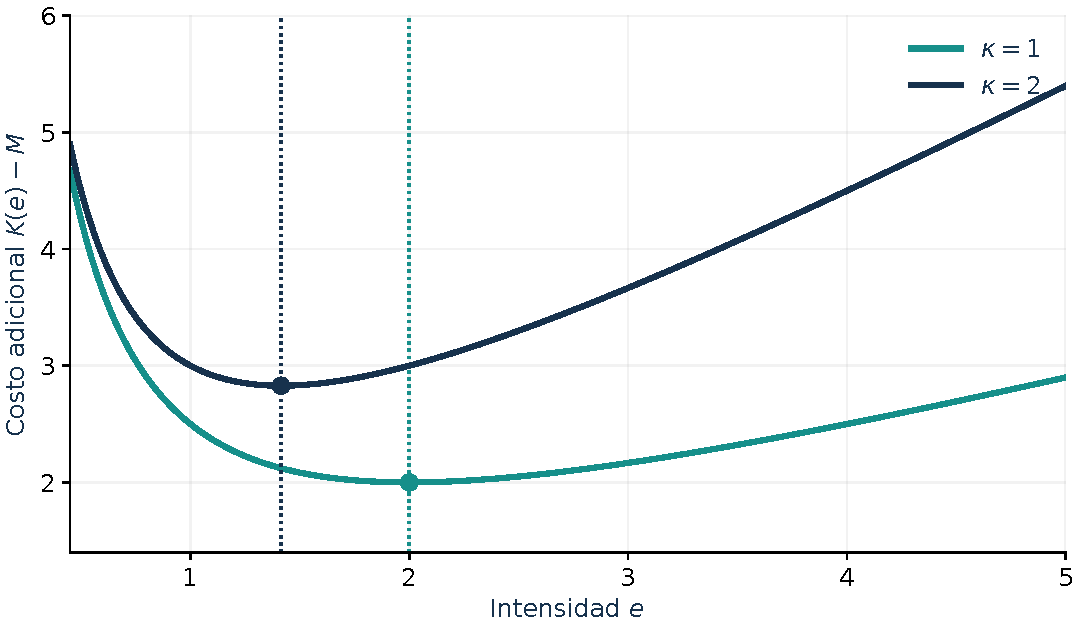
\includegraphics[width=\linewidth]{figures/cost_intensity.pdf}
\end{column}
\end{columns}
\notefoot{Escenario ilustrativo: $F=2$. Puntos: mínimos de cada curva. El costo mostrado excluye el componente fijo $M$.}
\end{frame}

\begin{frame}{3. Conjetura 1: intensidad, duración y costo}
\textbf{Bajo A1--A4, para $F>0$, $M\geq0$, $\kappa(p,C)>0$:}
\[
e^*=\sqrt{\frac{2F}{\kappa}},\quad
T^*=\sqrt{\frac{\kappa}{2F}},\quad
K^A=M+\sqrt{2F\kappa}.
\]
\par\vspace{2mm}
\centering
\renewcommand{\arraystretch}{1.45}
\begin{tabular}{lccc}
\toprule
Cambio supuesto & Intensidad & Duración & Costo\\
\midrule
$p$ aumenta, $\kappa_p>0$ & Disminuye & Aumenta & Aumenta\\
$C$ aumenta, $\kappa_C<0$ & Aumenta & Disminuye & Disminuye\\
\bottomrule
\end{tabular}
\par\vspace{3mm}
\[
\frac{\partial e^*}{\partial p}
=-\frac{\sqrt{2F}}{2\kappa^{3/2}}\kappa_p<0.
\]
\notefoot{Las comparaciones mantienen constantes los otros parámetros. Los signos sobre pobreza son condicionales a A4.}
\end{frame}

\begin{frame}{3. Mayor fricción reduce intensidad y prolonga duración}
\centering
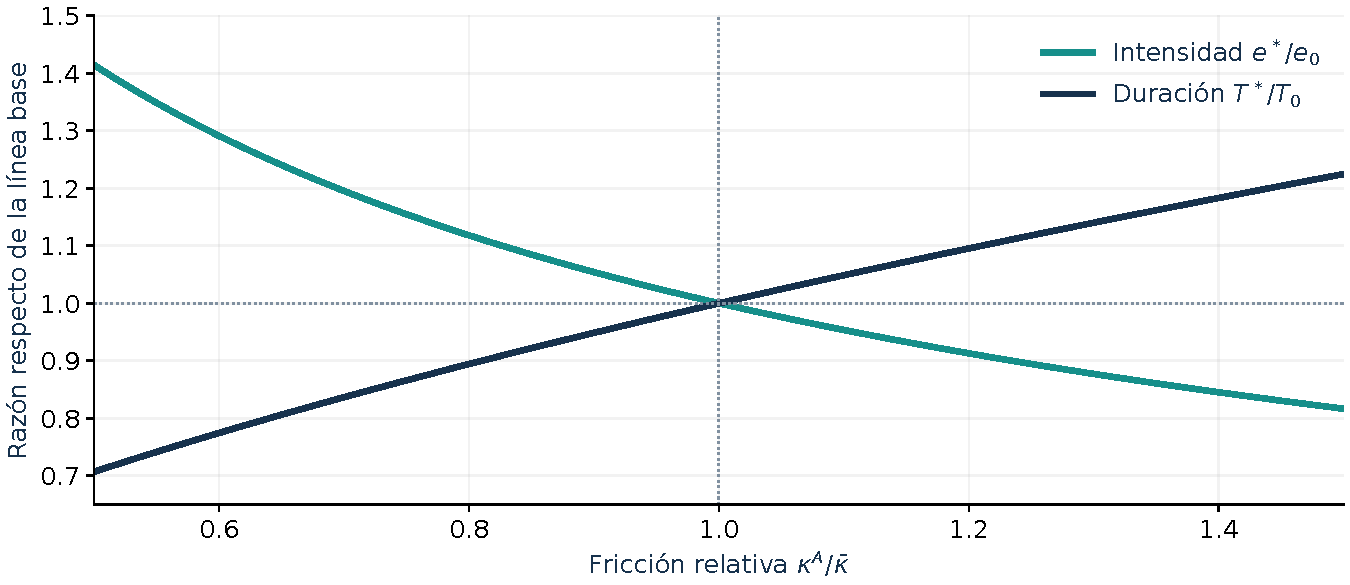
\includegraphics[width=.84\textwidth,height=5.3cm,keepaspectratio]{figures/speed_duration.pdf}
\lead{Si la fricción es 1.5 veces la referencia, $e^*/e_0\approx0.816$ y $T^*/T_0\approx1.225$.}
\notefoot{Escenarios teóricos, sin datos ni calibración al Perú. Las razones son $(\kappa^A/\bar\kappa)^{-1/2}$ y $(\kappa^A/\bar\kappa)^{1/2}$.}
\end{frame}

\begin{frame}{3. Conjetura 2: la condición exacta de sobrecosto}
\textbf{Bajo A1--A5, con $M,F$ iguales en ambas etapas:}
\[
R=\log\left(\frac{M+\sqrt{2F\kappa^A}}
{M+\sqrt{2F\kappa^V}}\right),\qquad
\boxed{R>0\iff\kappa^A>\kappa^V.}
\]
\lead{Una obra puede ser lenta y costosa, pero ajustarse a su presupuesto si sus dificultades fueron anticipadas.}
\begin{itemize}\setlength{\itemsep}{3mm}
\item Si $\kappa^V$ está fija, aumentar $p$ eleva $R$ bajo A4.
\item Si el presupuesto también incorpora el cambio de $p$, hay que estudiar ambos costos.
\end{itemize}
\notefoot{La duración total se convierte en retraso sólo al compararla con un plazo previsto.}
\end{frame}

\begin{frame}{3. Extensión: cuánto se incorpora en la previsión}
\[
\kappa^V(\lambda)=\lambda\kappa^A+(1-\lambda)\bar\kappa,
\qquad\lambda\in[0,1].
\]
\begin{itemize}\setlength{\itemsep}{3mm}
\item $\lambda=0$: presupuesto basado en una fricción genérica.
\item $0<\lambda<1$: incorporación parcial de condiciones locales.
\item $\lambda=1$: anticipación completa y $R=0$.
\end{itemize}
\lead{Si $\kappa^A>\bar\kappa$, una mayor incorporación reduce $R$.\\
La intensidad y la duración realizadas siguen dependiendo de $\kappa^A$.}
\notefoot{$\lambda$ es exógeno. Esta regla determinista permite comparar escenarios, no representa una expectativa racional ni una elección de información.}
\end{frame}

\begin{frame}{3. Anticipar mejor reduce la diferencia presupuestaria}
\centering
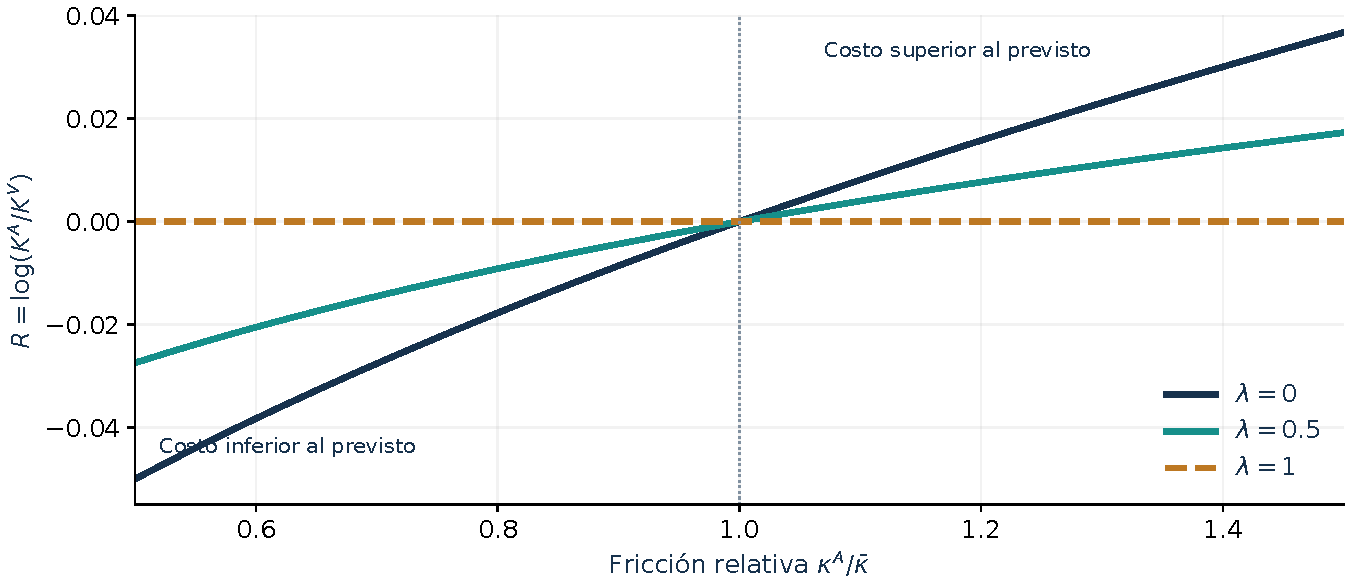
\includegraphics[width=.82\textwidth,height=4.9cm,keepaspectratio]{figures/overrun.pdf}
\lead{Con fricción superior a la referencia, $R$ baja al aumentar $\lambda$. Por debajo de la referencia, la variación negativa se acerca a cero.}
\notefoot{Escenario: $M=10$, $F=2$, $\bar\kappa=1$, unidades arbitrarias. $R$ se mide en logaritmos y no directamente en porcentajes.}
\end{frame}

\begin{frame}{3. El modelo y las medidas de la tesis}
\vspace{2mm}
\renewcommand{\arraystretch}{1.35}
\begin{tabular}{p{.37\textwidth}p{.55\textwidth}}
\toprule
\textbf{Modelo} & \textbf{Tesis: anexo 3}\\
\midrule
$e^*=1/T^*$ & (Devengado / costo actualizado) dividido por años desde el primer devengado.\\
$R=\log(K^A/K^V)$ & Logaritmo del costo actualizado sobre monto viable.\\
\bottomrule
\end{tabular}
\par\vspace{4mm}
\lead{La velocidad coincide sólo con gasto proporcional al progreso, proyecto completado y fechas físicas y financieras alineadas.}
\begin{itemize}
\item El costo actualizado puede incorporar cambios de alcance y no ser final.
\item Los proyectos en ejecución requieren tratar la censura.
\end{itemize}
\notefoot{Predicciones cualitativas: la equivalencia con registros administrativos requiere validación.}
\end{frame}

\begin{frame}{4. Capacidad, contexto y desempeño}
\textbf{Loayza et al. (2014), municipios peruanos}\\[1mm]
Personal profesional y educación se asocian con mayor ejecución; pobreza, con mayor proporción ejecutada en gasto corriente y de capital.
\par\vspace{3mm}
\textbf{Presbitero (2016), proyectos del Banco Mundial}\\[1mm]
Las expansiones de inversión se asocian con menor éxito. El efecto es pequeño y menor en países pobres y con escasez de capital.
\par\vspace{2mm}
\textbf{Gambina y Mazzola (2025), proyectos europeos}\\[1mm]
Calidad institucional y densidad poblacional se asocian con mayor velocidad; mayor PIB por habitante, con mayor duración.
\lead{La capacidad y el contexto importan. Estos resultados no establecen que más pobreza implique necesariamente mayor fricción.}
\notefoot{Loayza, p. 64; Presbitero, secciones 3--6; Gambina y Mazzola, secciones 3--4.}
\end{frame}

\begin{frame}{4. Modelos de costos y previsión inicial}
\textbf{Gurara et al. (2020): antecedente teórico próximo}\\[1mm]
Un contratista minimiza costos bajo incertidumbre y restricciones de absorción ligadas al tamaño del programa de inversión.
\par\vspace{3mm}
\textbf{Mohammadi Atashgah et al. (2022)}\\[1mm]
Optimizan tiempo y costo con modos, precedencias, incertidumbre y sobregiro.
\par\vspace{3mm}
\textbf{Espinoza y Presbitero (2022); Flyvbjerg et al. (2002)}\\[1mm]
Preparación e instituciones se relacionan con retrasos; la subestimación de costos también puede responder a incentivos estratégicos.
\lead{El modelo compara fricción prevista y realizada al elegir una intensidad continua. Los incentivos de subestimación quedan fuera de su alcance.}
\notefoot{Gurara: sección 2, pp. 4--6; Atashgah: pp. 262--264; Espinoza: sección 3; Flyvbjerg: conclusiones.}
\end{frame}

\begin{frame}{4. Búsqueda realizada y contribución delimitada}
\textbf{Búsqueda y revisión al 13/10/2026}\\[1mm]
Banco Mundial, FMI, JISE, arXiv y editoriales; revisión de diez PDF proporcionados, con siete antecedentes centrales.
\par\vspace{3mm}
\textbf{Comparación con los antecedentes más próximos}
\begin{itemize}\setlength{\itemsep}{2mm}
\item \textbf{Gurara:} contratista e insumos. \textbf{Aquí:} municipio e intensidad $e$.
\item \textbf{Atashgah:} actividades y modos. \textbf{Aquí:} solución analítica continua.
\item \textbf{Previsión:} comparar $\kappa^A$ y $\kappa^V$ separa costo alto y sobrecosto.
\end{itemize}
\lead{Aporte propuesto: integrar fricción distrital, intensidad óptima y anticipación presupuestaria. Mejorar la previsión puede reducir el sobrecosto sin acelerar la obra.}
\notefoot{Alcance: síntesis y adaptación respecto de los textos examinados. No se identificó allí esta combinación exacta; no se afirma originalidad exhaustiva. Registro: literatura\_busqueda.md.}
\end{frame}

\begin{frame}{5. Plan de demostración, simulación y Lean}
\begin{itemize}\setlength{\itemsep}{4mm}
\item \textbf{Demostrar:} óptimo único, comparativas estáticas, condición exacta $R>0$ y efecto de $\lambda$ para ambas direcciones de la brecha.
\item \textbf{Simular:} $\kappa^A/\bar\kappa\in[0.5,1.5]$ y $\lambda\in\{0,0.5,1\}$. El script adjunto reproduce los gráficos y verifica resultados numéricos. SymPy es el siguiente paso.
\item \textbf{Lean:} caracterización del mínimo, orden de resultados y condición de sobrecosto, con dominios explícitos.
\end{itemize}
\[
K(e;\kappa)-K(q;\kappa)=\frac{\kappa}{2e}(e-q)^2\geq0,
\qquad q=\sqrt{2F/\kappa}.
\]
\notefoot{La identidad ofrece una ruta de prueba algebraica. Lean y la demostración manuscrita completa están pendientes.}
\end{frame}

\begin{frame}{5. Riesgos y alcance de la interpretación}
\textbf{Riesgo principal: medición}\\[1mm]
El avance financiero puede separarse del físico. El costo actualizado puede incluir cambios de alcance.
\par\vspace{4mm}
\textbf{Riesgo del mecanismo}\\[1mm]
El signo $\kappa_p>0$ puede no describir los datos o desaparecer al considerar otros controles.
\par\vspace{4mm}
\textbf{Respuesta prevista}\\[1mm]
Documentar límites y mantener las conclusiones condicionales. Formalizar raíces y logaritmos con todos sus dominios.
\lead{Reducir la fricción puede mejorar la ejecución. Anticiparla mejor puede reducir la diferencia presupuestaria sin modificar la duración realizada.}
\end{frame}

\appendix
\begin{frame}{Referencias consultadas (1/2)}
\small
\begin{itemize}\setlength{\itemsep}{3mm}
\item Bolo Añorga, C. A. y Roque Tinta, I. M. (2026). \emph{Pobreza y desempeño en la inversión pública en el Perú}. Plan de tesis, 27/09.
\item Loayza, N. V., Rigolini, J. y Calvo-González, O. (2014). More than you can handle: Decentralization and spending ability of Peruvian municipalities. \emph{Economics \& Politics, 26}(1), 56--78. \href{https://doi.org/10.1111/ecpo.12026}{DOI}.
\item Presbitero, A. F. (2016). Too much and too fast? Public investment scaling-up and absorptive capacity. \emph{Journal of Development Economics, 120}, 17--31. \href{https://doi.org/10.1016/j.jdeveco.2015.12.005}{DOI}.
\item Gurara, D., Kpodar, K., Presbitero, A. F. y Tessema, D. (2020). \emph{On the Capacity to Absorb Public Investment: How Much is Too Much?} FMI WP/20/48. Texto completo revisado; publicado en \emph{World Development} (2021).
\end{itemize}
\end{frame}

\begin{frame}{Referencias consultadas (2/2)}
\small
\begin{itemize}\setlength{\itemsep}{3mm}
\item Gambina, D. y Mazzola, F. (2025). The Determinants of the Implementation Speed of Cohesion Projects in Europe: A Regional and Project-level Analysis. \emph{Open Economies Review}. \href{https://doi.org/10.1007/s11079-025-09819-3}{DOI}.
\item Espinoza, R. y Presbitero, A. F. (2022). Delays in public investment projects. \emph{International Economics, 172}, 297--310. \href{https://doi.org/10.1016/j.inteco.2021.10.002}{DOI}.
\item Mohammadi Atashgah, K. et al. (2022). Developing a model for time-cost trade-off optimization problem considering overdraft issue in uncertain environments. \emph{Journal of Industrial and Systems Engineering, 14}(3), 259--279. \href{https://www.jise.ir/article_154961.html}{Texto completo}.
\item Flyvbjerg, B., Holm, M. K. S. y Buhl, S. L. (2002). Underestimating costs in public works projects: Error or lie? \emph{Journal of the American Planning Association, 68}(3), 279--295. \href{https://doi.org/10.1080/01944360208976273}{DOI}. Copia del autor: arXiv:1303.6604.
\end{itemize}
\end{frame}
\end{document}
